\section{The Disaster Scenario}

\noindent We consider a disaster scenario involving a satellite, containing radioactive fuel, that has crashed in a sub-urban area (see Section \ref{atomic} to see how this helps implement a credible mixed-reality game). While debris is strewn around a large area, damaging buildings and causing accidents and injuring civilians, radioactive discharge from the debris is gradually spreading over the area, threatening to contaminate food reserves and people. Hence, emergency services, voluntary organisations, and the military are deployed to help evacuate the casualties and resources before these are engulfed by  radioactive cloud.  In what follows, we model this scenario formally and then describe the optimisation problem faced by the actors (i.e., including emergency services, volunteers, medics, and soldiers) in trying to save as many lives and resources as they can.

\subsection{Formal Model}
\noindent Let $G$ denote a grid overlaid on top of the disaster space, and the satellite and actors are located at various coordinates $(x,y) \in G$ in this grid. The set of field responders be denoted as $i_1, \cdots, i_n \in I$ and the set of rescue tasks as  $t_1,\cdots, t_m\in T$.  As responders enact tasks, they may become tired or get injured. Hence, we assign each responder  a health level $h_i\in [0,100]$. Moreover, each responder will have  a specific role  $r \in Roles$ (e.g., fire brigade, soldier, or medic) and this will determine the capabilities he or she has and therefore the tasks he or she can perform. We denote as $Roles(i)$ the role of responder $i$. In turn, to complete a given task $t$,  a set of responders $I' \subseteq I$ with specific roles $R_t \subseteq R$ is required. Thus, a task can only be completed by a team of responders $I'$ if $\{Roles(i) | i \in I'\} = R_t$. 

Given this model, we next formulate the optimisation problem faced by the responders (and later solved in Section \ref{sec:algo}). To this end, we propose a Multi-Agent Markov Decision Process (MMDP)~\cite{?} that captures the uncertainties of the radiative cloud and the responders' behaviours. Specifically, we model the spreading of the radiative cloud as a random process over the spatial space and allow the responders' actions to be failed or delayed during the rescue process. Other existing models for rescue tasks such as CFSTP~\cite{?} and HTSSC~\cite{?} cannot be applied to our problem as they usually require the process of task executions to be deterministic. They need to explicitly model the time limit of a task and the duration of completing a task by the responders as spatial and temporal constraints, which are stochastic in our domain. Instead, in the MMDP model, we represent the task executions as stochastic processes of state transitions. Thus, the uncertainties of the radiative cloud and the responders' behaviours can be straightforwardly captured with transition probabilities. Additionally, modeling the problem as a MMDP enables us to use many sophisticated algorithms that have already been developed in the literature.

\subsection{Radiation Cloud Modelling}\label{sec:radiation}
\noindent The radiation cloud is assumed to be monitored using a number of sensors on the ground (within the disaster space) that collect readings of the radiation cloud intensity and wind velocity every minute of the game. These sensors can be at fixed locations or held by mobile agents.  The radiation cloud diffusion process is modelled in a standard way by a nonlinear Markov field stochastic differential equation,  
\begin{eqnarray*}
\frac{D \text{Rad}({\bf z}, \tau)}{D \tau}=\kappa \triangledown^2 \text{Rad}({\bf z},\tau)-\text{Rad}({\bf z},\tau)\triangledown \cdot {\bf w}({\bf z},\tau)+\sigma({\bf z},\tau)
\end{eqnarray*}
where $D$ is the material derivative, $\text{Rad}({\bf z},\tau)$ is the radiation cloud intensity at location ${\bf z}$ at time $\tau$, $\kappa$ is a fixed diffusion coefficient and $\sigma$ is the radiation source(s) emission rate. The diffusion equation is solved on a regular grid defined across the environment with grid coordinates $G$ (as defined in Section \ref{sec:model}).  Furthermore, the grid is solved at discrete time instances $\tau$.  The cloud is driven by wind forces which vary both spatially and temporally.  These forces induce anisotropy into the cloud diffusion process which is proportional to the wind velocity, ${\bf w}({\bf z},\tau)$.  The wind velocity is drawn from two independent Gaussian processes (GP), one GP for each Cartesian coordinate axis, $w_i({\bf z},\tau)$, of ${\bf w}({\bf z},\tau)$.  The GP captures both the spatial distribution of the wind velocity and the dynamic process resulting from shifting wind patterns such as short term gusts and longer term variations. 

% In our simulation, each spatial wind velocity component is modelled by a squared-exponential GP covariance function, $K$, with fixed input and output scales (although any covariance function can be substituted). Furthermore, as wind conditions may change over time we introduce a temporal correlation coefficient, $\rho$, to the covariance function.  Thus, for a single component, $w_i$, of ${\bf w}$, defined over grid $G$ at times $\tau$ and $\tau^\prime$, the wind process covariance function is, $\text{Cov}(w_i(G,\tau),w_i(G,\tau^\prime))=\rho(\tau,\tau^\prime) K(G,G)$.  We note that, when $\rho=1$ the wind velocities are time invariant (although spatially variant).  Values of $\rho<1$ model wind conditions that change over time.

Using the above model, we are able to create a moving radiation cloud, thus posing a real challenge both for the HQ (agent and commander) and the responders on the ground, as predictions they can make of where the cloud will move to will be prone to uncertainty both to the simulated wind speed and direction. 


%(\textbf{Steve: in the platform we take the `real' values from the diffusion process i believe. Does the above capture this? We will say that we will add the features you mention below to a future version of the platform where we aim to do both situational awareness and rescue. Add a sentence above to conclude where we took the values from and the process takes into account the  location of radiation source. Also, your notation clashes with the notations in the scenario and Feng's algorithm - please try to align.}
%The cloud intensity and wind velocity are measured by {\it monitor agents} equipped with geiger-counters and anemometers.  These agents are directed to take measurements with greatest information gain in the radiation cloud intensity.  The measurements are folded into the EKF and this refines estimates of the radiation cloud across the grid.  Figure~\ref{radiation_screen_shots} shows example cloud simulations for slow varying (i.e. $\rho=0.99$) and gusty (i.e. $\rho=0.90$) wind conditions.  Figure~\ref{radiation_screen_shots}(a) shows slow varying wind conditions in which case the radiation cloud can be interpolated accurately using sparse sensor measurements and the LFM model.  Alternatively, during gusty conditions the radiation cloud model is more uncertain far from the locations where recent measurements have been taken, as shown in Figure~\ref{radiation_screen_shots}(b).
%
%\begin{figure}[ht] \begin{center}
%    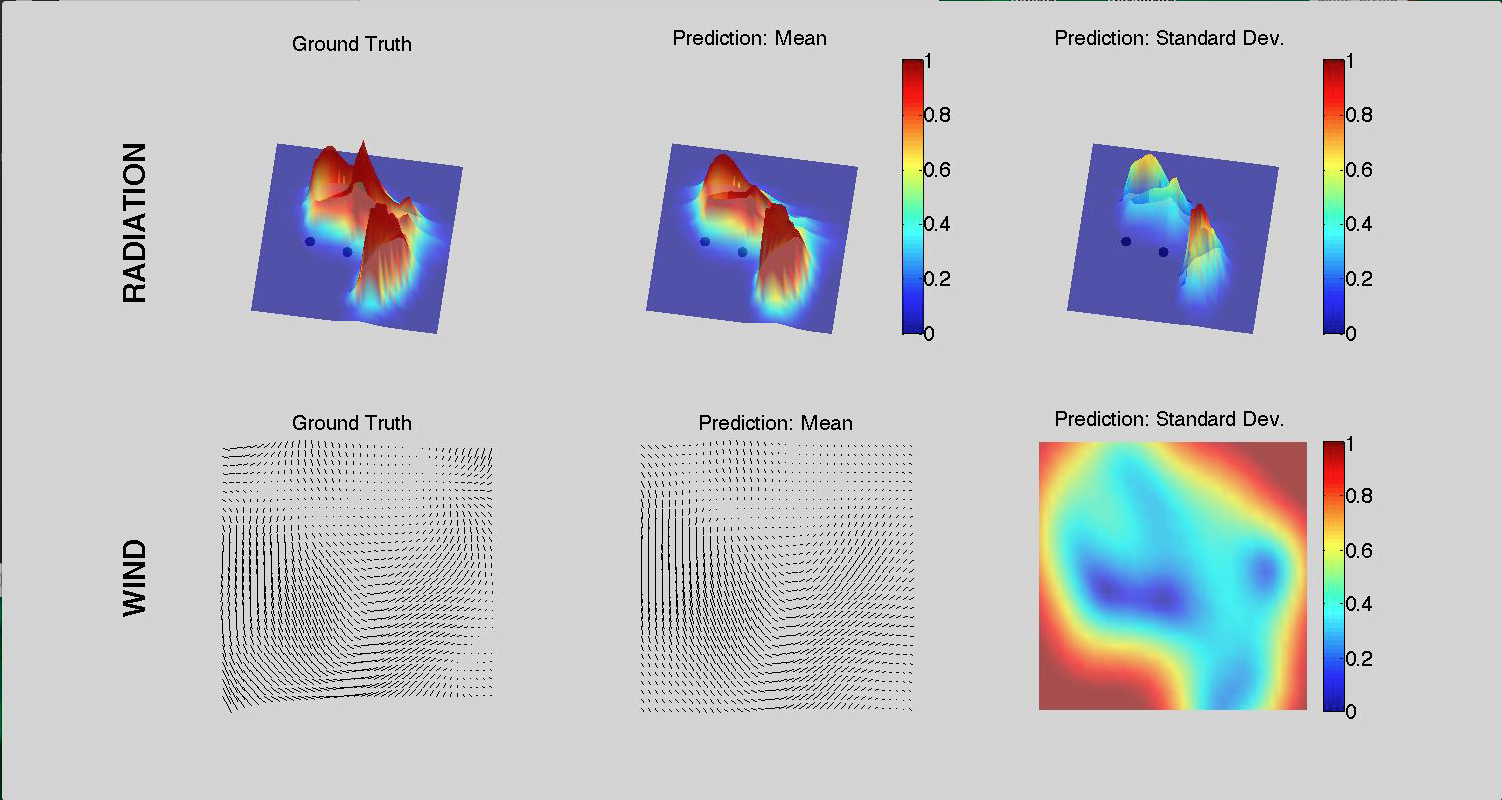
\includegraphics[width=0.45\textwidth]{figures/radiation_ss_calm.png}\\
%    (a) Slowly varying wind conditions\\ \ \\
%    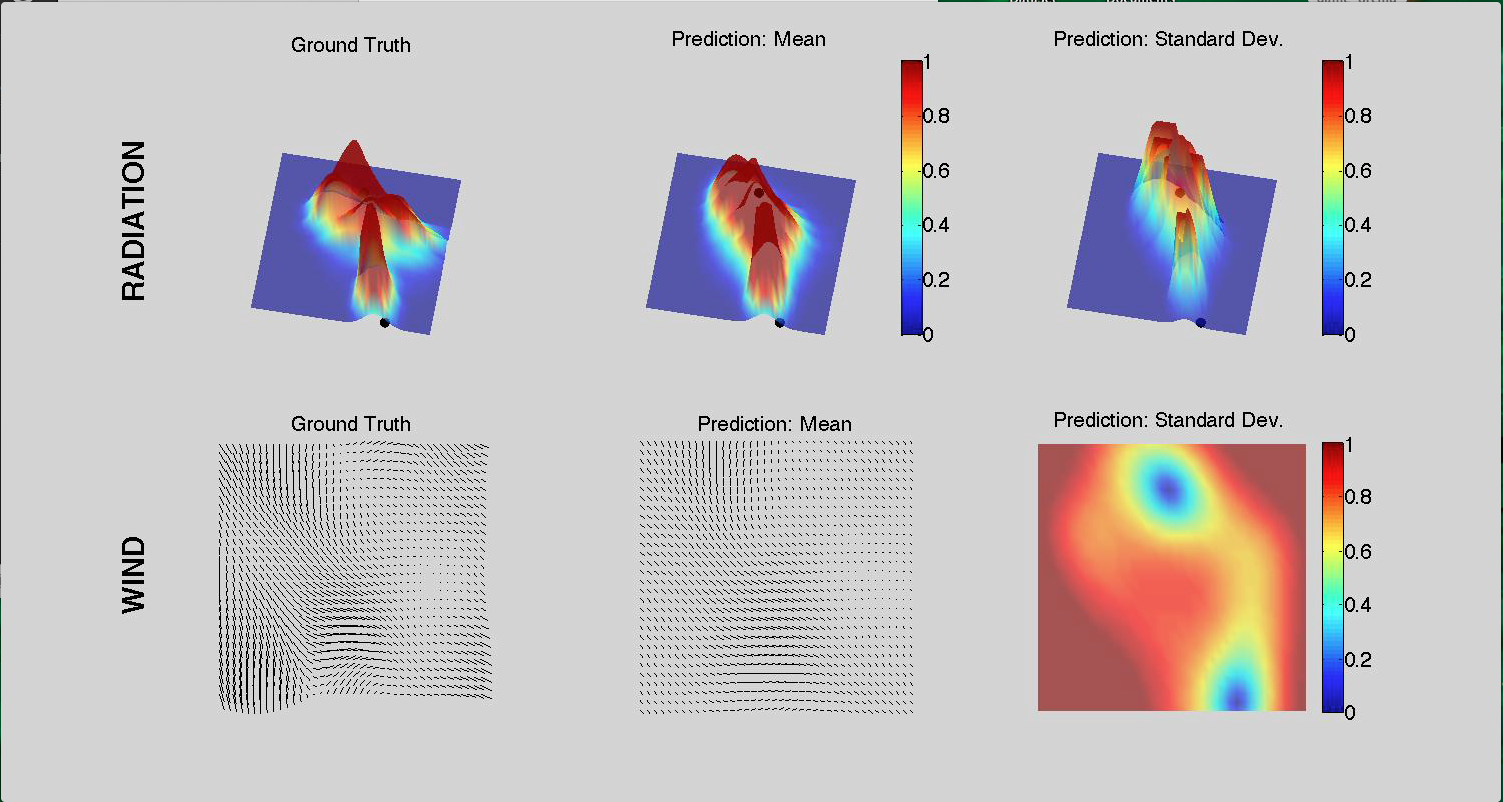
\includegraphics[width=0.45\textwidth]{figures/radiation_ss_gust.png}\\
%    (b) Gusty wind conditions 
%\caption{\label{radiation_screen_shots} Radiation and wind simulation ground truth and EKF estimates obtained using measurements from monitor agents (black dots).  Left most panes are ground truth radiation and wind conditions, the middle panes are corresponding estimates and right most panes are state uncertainties:  (a) Invariant and (b) gusty wind conditions.}
%\end{center}
%\end{figure}

\subsection{The Optimisation Problem}
\label{sec:model}
\noindent Previous agent-based models for team coordination in disaster response typically assume deterministic task executions and environments \cite{ramchurn:etal:2010,Scerri2005}. However, in order to evaluate agent-guided coordination in a real-world environment, it is important to consider uncertainties due to player behaviours and the environment (as discussed in the previous section). Given this, we propose a new representation for the task allocation problem in disaster response that does take into account such uncertainties. More specifically, we represent this problem using an MMDP that captures the uncertainties of the radioactive cloud and the responders' behaviours. We model the spreading of the radioactive cloud as a random process over the disaster space and allow the actions requested from the responders to  fail (because they decline to go to a  task) or incur delays (because they are too slow) during the rescue process. Thus in the MMDP model, we represent  task executions as stochastic processes of state transitions, while the uncertainties of the radioactive cloud and the responders' behaviours can be easily captured with transition probabilities.  More formally, the MMDP is
represented by tuple $\mathcal{M} = \langle I, S, \{A_i\}, P, R
\rangle$, where $I$ is the set of actors as defined in the previous
section,  $S$ is the state space, $A_i$ is a set of responder
$p_i$'s actions, $P$ is the transition function, and $R$ is the
reward function. We elaborate on each of these below.

In more detail, $S= S^G_r \times S_{p_1} \times \cdots \times
S_{p_n} \times S_{t_1} \times \cdots \times S_{t_m}$ where $S^G_r =
\{l_{(x,y)}| (x, y) \in G\}$ is the state variable of the
radioactive cloud that specifies the radioactive level
$l_{(x,y)}\in[0, 100]$ at every point $(x, y)\in G$. $S_{p_i} =
\langle h_i, (x_i, y_i), t_j \rangle$ is the state variable for
each responder $p_i$ that specifies her health level
$h_i\in[0, 100]$, her present position $(x_i, y_i)$, and the task
$t_j$ she is carrying out. $S_{t_j} = \langle {\tt st_j}, (x_j, y_j)
\rangle$ is then the state variable for task $t_j$ to specify its
status ${\tt st_j}$ (i.e., the target is picked up, dropped off, or idle) and position $(x_j, y_j)$. 

The three types of actions  (in set $A_i$) a responder can take
are: (i) {\em stay} in the current location $(x_i, y_i)$, (ii) {\em
move} to the 8 neighbouring locations, or (iii) {\em complete} a
task located at $(x_i, y_i)$. A joint action $\vec{a}=\langle a_1,
\cdots, a_n \rangle$ is a set of actions where $a_i\in A_i$, one
for each responder (a responder may just \emph{stay} at its current
position if it has no targets to rescue). The transition function
$P$ is defined in more detail as: $P= P_r \times P_{p_1} \times
\cdots \times P_{p_n} \times P_{t_1} \times \cdots \times P_{t_m}$
where:
\begin{itemize}
    \itemsep=-2pt
    \item $P_r(s'_r|s_r)$ is the probability the radioactive
        cloud spreads from state $s_r\in S^G_r$ to $s'_r\in
        S^G_r$. It captures the uncertainty of the  radiation
        levels in the environment due to  noisy sensor readings
        and the variations in wind speed and direction.
    \item $P_{p_i}(s'_{p_i}|s, a_i)$ is the probability
        responder $p_i$ transitions to a new state $s'_{p_i}\in
        S_{p_i}$ when executing action $a_i$. For example, when
        a responder is asked to go to a new location,  she
        may not end up there because  she is tired,
        gets injured, or receives radiation doses that are life
        threatening.
    \item $P_{t_j}(s'_{t_j}|s, \vec{a})$ is the probability
        of task $t_j$ being completed. A task $t_j$ can only be completed by a
        team of responders with the required types ($\Theta_{t_j}$) located at the
        same position as $t_j$.
\end{itemize}

Now,  if  $t_j$ is completed (i.e., in ${\tt st_j}\in S_{t_j}$, the
status ${\tt st_j}$ is marked as ``dropped off'' and its position $(x_j,
y_j)$ is within a safe zone), the team will be rewarded using
function $R$. The team is penalised if a responder $p_i$ gets
injured or receives a high dose of radiation (i.e., in $s_{p_i}$,
the health level $h_i$ is 0). Moreover, we attribute a cost to each
of the responders' actions since  each  action requires them to
exert some effort (e.g., running or carrying objects).


Give the above definitions, a policy for the MMDP is a mapping from
states to joint actions, $\pi: S \rightarrow \vec{A}$ so that the
responders know which actions to take given the current state of
the problem. The quality of a policy $\pi$ is  measured by
its expected value $V^\pi$, which can be computed recursively by
the Bellman equation:
\begin{equation}
  V^\pi(s^\tau) = R(s^\tau, \pi(s^\tau)) + \!\!\!\sum_{s^{\tau+1}\in S}\!\!\!
  P(s^{\tau+1}|s^\tau, \pi(s^t)) V^\pi(s^{\tau+1})
\end{equation}
where $\tau$ denotes the current time point and $\pi(s^\tau)$ is a joint action given $s^\tau$. The goal of solving
the MMDP is to find an optimal policy $\pi^*$ that maximises the
expected value with the initial state $s^0$, $\pi^* =
\arg\max_{\pi} V^\pi(s^0)$.

At each decision step, we assume the planning agent can fully
observe the state of the environment $s$ by collecting sensor
readings of the radioactive cloud and GPS locations of the
responders. Given a policy $\pi$ of the MMDP, a joint action
$\vec{a}=\pi(s)$ can be selected and broadcast to the responders
(as mentioned earlier).

